% =============================================================================
% Unbranded copy (no Mustang Capital branding)
% AI Infrastructure and the Concentration of Credit Risk in U.S. IG Markets
% Research cutoff: 13 November 2026
% Compile: xelatex main_unbranded.tex && xelatex main_unbranded.tex
% =============================================================================
\documentclass[10pt,letterpaper]{article}

% --- layout -----------------------------------------------------------------
\usepackage[margin=0.75in,top=0.78in,bottom=1.0in,headheight=20pt,headsep=10pt,footskip=32pt]{geometry}
\usepackage{amsmath}
\usepackage{microtype}
\usepackage{setspace}
\setstretch{1.07}
\usepackage{enumitem}
\setlist[itemize]{leftmargin=1.1em,itemsep=0.28em,parsep=0.05em,topsep=0.25em}
\setlist[enumerate]{leftmargin=1.25em,itemsep=0.28em,parsep=0.05em,topsep=0.25em}

% --- fonts ------------------------------------------------------------------
% Body: Times New Roman. Headings: Cambria.
\usepackage{fontspec}
\setmainfont{Times New Roman}[
  Path=/System/Library/Fonts/Supplemental/,
  Extension=.ttf,
  UprightFont=*,
  BoldFont=* Bold,
  ItalicFont=* Italic,
  BoldItalicFont=* Bold Italic,
  Ligatures=TeX
]
\newfontfamily\headingfont{Cambria}[
  Path=/Applications/Microsoft Word.app/Contents/Resources/DFonts/,
  UprightFont=Cambria.ttc,
  BoldFont=Cambriab.ttf,
  ItalicFont=Cambriai.ttf,
  BoldItalicFont=Cambriaz.ttf,
  Ligatures=TeX
]

% --- colour -----------------------------------------------------------------
\usepackage{xcolor}
\definecolor{ink}{HTML}{1C1C1C}
\definecolor{navy}{HTML}{881810}
\definecolor{muted}{HTML}{5A5A5A}
\definecolor{lightline}{HTML}{D8D8D8}
\color{ink}

% --- graphics / tables ------------------------------------------------------
\usepackage{graphicx}
\usepackage{booktabs}
\usepackage{caption}
\captionsetup{
  font={small},
  labelfont={bf,color=navy},
  textfont={color=ink},
  skip=5pt,
  justification=raggedright,
  singlelinecheck=false
}
\usepackage{float}
\usepackage{placeins}
\usepackage{needspace}

% --- headers / titles -------------------------------------------------------
\usepackage{fancyhdr}
\usepackage{titlesec}
\usepackage{tikz}
\usetikzlibrary{arrows.meta,positioning}
\usepackage{hyperref}
\hypersetup{
  colorlinks=true,linkcolor=navy,urlcolor=ink,citecolor=navy,
  pdftitle={AI Infrastructure and the Concentration of Credit Risk in U.S. Investment Grade Bond Markets},
  pdfauthor={Vinesh Ranganathan},
  pdfsubject={Global Macro research outlook},
  pdfkeywords={investment grade, hyperscalers, duration risk, credit markets, AI infrastructure}
}
% Clickable reference URL with an explicit wrap-safe display line
\newcommand{\sourcelink}[2]{%
  \par\nobreak\vspace{0.05em}%
  \noindent{\footnotesize\color{ink}\href{#1}{\ttfamily #2}}\par}

\pagestyle{fancy}
\fancyhf{}
\renewcommand{\headrulewidth}{0.4pt}
\renewcommand{\footrulewidth}{0.35pt}
\renewcommand{\headrule}{\hbox to\headwidth{\color{lightline}\leaders\hrule height \headrulewidth\hfill}}
\renewcommand{\footrule}{\hbox to\headwidth{\color{lightline}\leaders\hrule height \footrulewidth\hfill}}
\fancyhead[L]{\small\headingfont\color{navy}\textbf{Global Macro}}
\fancyhead[R]{\small\headingfont\color{navy}\textbf{Research Outlook}}
\fancyfoot[L]{\footnotesize\color{muted}13 November 2026}
\fancyfoot[C]{\footnotesize\color{muted}Global Macro}
\fancyfoot[R]{\footnotesize\color{muted}\thepage}

\titleformat{\section}
  {\normalsize\headingfont\bfseries\color{navy}}{\thesection.}{0.5em}{}
  [\vspace{0.22em}{\color{lightline}\titlerule[0.4pt]}\vspace{0.42em}]
\titleformat{\subsection}
  {\small\headingfont\bfseries\color{navy}}{\thesubsection}{0.5em}{}
\titlespacing*{\section}{0pt}{1.15em}{0.45em}
\titlespacing*{\subsection}{0pt}{0.85em}{0.32em}
\titleformat{\paragraph}[runin]
  {\footnotesize\bfseries\color{ink}}{}{0em}{}[.]
\titlespacing*{\paragraph}{0pt}{0.55em}{0.4em}
\setlength{\parindent}{1.15em}
\setlength{\parskip}{0pt}

\titleformat{name=\section,numberless}
  {\normalsize\headingfont\bfseries\color{navy}}{}{0em}{}
  [\vspace{0.22em}{\color{lightline}\titlerule[0.4pt]}\vspace{0.42em}]

\clubpenalty=10000
\widowpenalty=10000
\displaywidowpenalty=10000
\raggedbottom

% --- citation helpers (numbered sources) ------------------------------------
\newcommand{\src}[1]{{\scriptsize\textcolor{navy}{[#1]}}}

\newcommand{\exhibitsource}[1]{%
  \vspace{0.1em}{\footnotesize\color{muted}#1\par}\vspace{0.22em}}

\newcommand{\exhibitblock}[4]{%
  \par\nobreak
  \noindent{\footnotesize\headingfont\bfseries\color{navy}#3}\par\vspace{0.28em}%
  \nobreak
  \noindent\includegraphics[width=#1\textwidth]{figures/#2}\par
  \nobreak
  \exhibitsource{#4}%
}

\newcommand{\thinrule}{\noindent{\color{lightline}\rule{\textwidth}{0.4pt}}\par}
\newcommand{\navyrule}{\noindent{\color{navy}\rule{\textwidth}{1.15pt}}\par}
\newcommand{\defsig}[2]{%
  \par\vspace{0.35em}%
  \noindent{\footnotesize\textbf{\color{navy}Definition.}\ #1\par}%
  \vspace{0.15em}%
  \noindent{\footnotesize\textbf{\color{navy}Significance.}\ #2\par}%
  \vspace{0.45em}%
}

\begin{document}
\thispagestyle{empty}

% =============================================================================
% COVER
% =============================================================================
\noindent
\begin{minipage}[c]{0.58\textwidth}
  \vspace{1pt}
  {\normalsize\headingfont\bfseries\color{navy}GLOBAL MACRO}\\[0.18em]
  {\footnotesize\color{muted}Research Outlook}
\end{minipage}%
\hfill
\begin{minipage}[c]{0.38\textwidth}
  \vspace{1pt}
  \raggedleft
  {\footnotesize\color{muted}13 November 2026}
\end{minipage}

\vspace{0.3em}
\navyrule
\vspace{0.35em}

% Title: even two-line stack with fixed leading
\noindent{\headingfont\fontsize{16}{18.5}\selectfont\bfseries\color{ink}%
AI Infrastructure and the Concentration of Credit Risk\\
in U.S.\ Investment Grade Bond Markets\par}

\vspace{0.7em}
\noindent{\headingfont\scriptsize\bfseries\color{navy}RESEARCH QUESTION}\\[0.42em]
{\setlength{\baselineskip}{14pt}%
\noindent{\fontsize{10.75}{14}\selectfont\color{ink}%
Does hyperscaler debt contribute disproportionately to interest-rate sensitivity
in U.S.\ investment-grade credit portfolios relative to its index market-value
weight, and what explains this exposure?\par}}

\vspace{0.55em}
\noindent
\begin{minipage}[c]{0.72\textwidth}
  \vspace{0pt}
  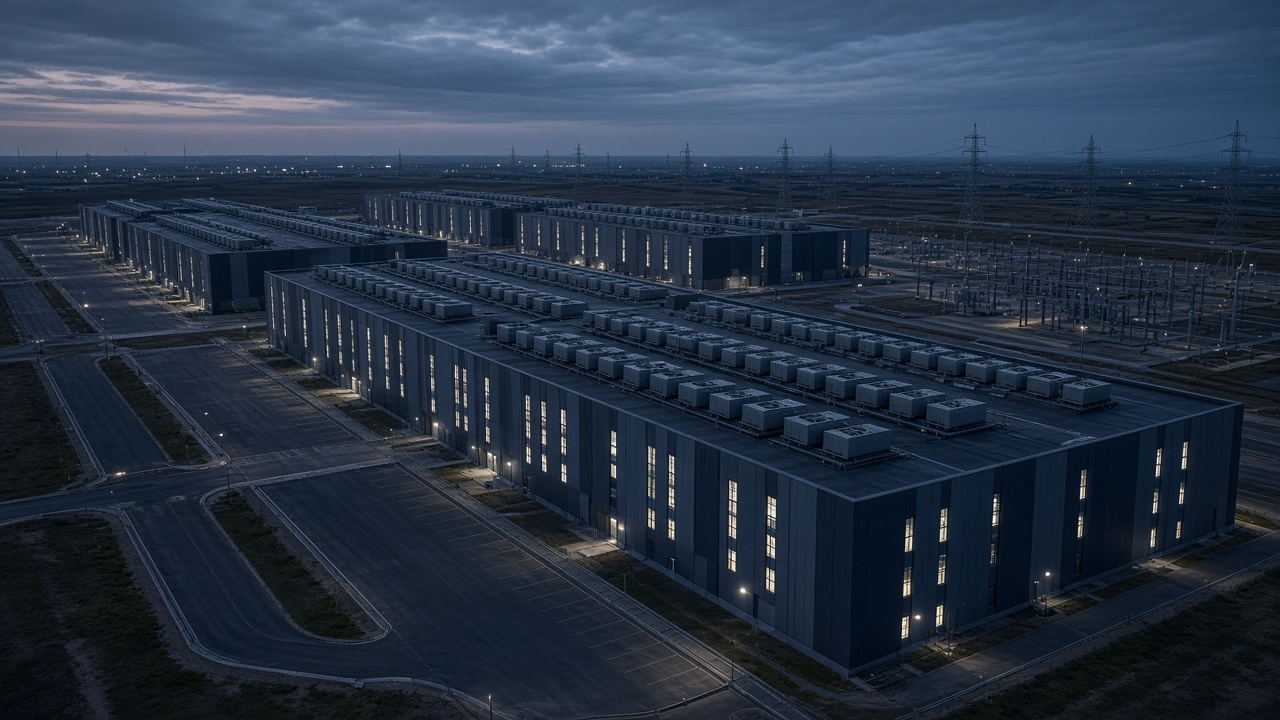
\includegraphics[width=\linewidth]{figures/cover_hyperscale_campus.jpg}
\end{minipage}%
\hfill
\begin{minipage}[c]{0.24\textwidth}
  \vspace{0pt}
  {\headingfont\scriptsize\bfseries\color{navy}AUTHOR}\\[0.35em]
  {\footnotesize\bfseries\color{ink}Vinesh Ranganathan}\\[0.22em]
  {\scriptsize\color{muted}Co-Lead, Global Macro}\\[0.12em]
  {\scriptsize\color{muted}Third-Year Computer Science Student}\\[0.12em]
  {\scriptsize\color{muted}Western University}
\end{minipage}

\vspace{0.75em}
\noindent{\headingfont\footnotesize\bfseries\color{navy}KEY FINDINGS}\\[-0.42em]
\thinrule
\vspace{0.28em}
\begin{enumerate}[leftmargin=1.2em,itemsep=0.2em,parsep=0em,topsep=0em,label={\footnotesize\textcolor{navy}{\textbf{\arabic*.}}}]
  \item {\small\textbf{Duration-risk exposure exceeds benchmark market weight.} As of about September~2026, Amazon, Alphabet, Microsoft, Meta and Oracle were 4.85\% of Bloomberg US Corporate Index market value and 6.3\% of its interest-rate (duration) risk, about 1.3$\times$ their weight (2.67\% / 3.6\% at end-2024). \src{10} Absolute shares rose; the relative multiple was broadly stable. Index holdings average 8.4 years versus 6.4 for the index; 2025--26 USD new issues averaged 8.9 years. \src{2}\src{10}}
  \item {\small\textbf{Registered issuance has surged.} SEC-registered volume rose from \$14\,bn in 2023 to \$284\,bn in 2026 (through 13~Nov). In Jan--Sep~2026, USD issuance by the five was 7.2\% of all US corporate bond supply and 10.4\% of IG supply in 3Q26. \src{2}\src{8}}
  \item {\small\textbf{Capex now absorbs nearly all operating cash flow.} Trailing twelve-month capex is \$691\,bn against \$724\,bn of operating cash flow. Oracle and Amazon are free-cash-flow negative (capex/OCF 1.61 and 1.28); Alphabet, Meta and Microsoft remain self-funding with less spare cash. \src{1}}
  \item {\small\textbf{Relative pricing gaps have widened versus rating-bucket OAS.} For 8--12 year new issues, Treasury spreads exceed same-rating ICE OAS by about +27\,bp (Amazon), +28\,bp (Alphabet), +93\,bp (Meta) and +194\,bp (Oracle); Microsoft still prices inside the AA bucket. Gaps are indicative comparisons, not measured concessions. \src{2}\src{4}}
  \item {\small\textbf{Near-term maturities are modest; sensitivity sits in long paper.} Contractual maturities over the next three years total \$60\,bn. A hypothetical +100\,bp rate and +100\,bp spread shock implies about an 18\% first-order price decline on the 2025--26 issuance book. \src{1}\src{2}}
\end{enumerate}

\clearpage
\pagenumbering{arabic}

% =============================================================================
\section{Market Outlook and Research Context}
% =============================================================================

AI-infrastructure financing has increased the market presence of a concentrated group of long-duration investment-grade borrowers: Amazon, Alphabet, Microsoft, Meta and Oracle. Their contribution to benchmark interest-rate sensitivity exceeds their market-value weight, while rising capital expenditure is changing issuer financing requirements. \src{1}\src{10} The vulnerabilities are not uniform. Near-term contractual maturities remain relatively manageable, and balance-sheet resilience differs substantially across issuers. The immediate market concern is concentration and absorption of long-duration credit exposure, together with issuer-specific financing pressure.

This note is an exploratory Global Macro research outlook. It documents market structure and quantifies concentration and sensitivity where public data allow. It is organised around three ideas:
\begin{enumerate}[leftmargin=1.2em,itemsep=0.2em]
  \item \textbf{What has changed?} Rapid debt issuance and a larger contribution to credit-market duration exposure.
  \item \textbf{Why does it matter?} Long-duration financing, capital intensity, relative spread pricing and uneven issuer resilience.
  \item \textbf{What happens under tighter conditions?} Potential market repricing, higher financing costs and theoretical transmission across capital-market participants.
\end{enumerate}

Published Bloomberg-based estimates place the five at 4.85\% of Bloomberg US Corporate Index market value and 6.3\% of its interest-rate duration risk as of about September~2026, versus 2.67\% and 3.6\% at end-2024. \src{10} Absolute market presence and duration-risk contribution both increased; the relative overrepresentation remained about 1.3$\times$ (1.35$\times$ in 2024; 1.30$\times$ in 2026). Independently, SEC filings show that registered issuance has jumped by an order of magnitude, new notes are long-duration, and new-issue Treasury spreads have moved away from rating-bucket ICE OAS averages, most clearly for Oracle and Meta. \src{2}\src{4} Capex now runs close to operating cash flow across the group, so external funding demand is structural for as long as the build continues. \src{1}

% =============================================================================
\section{Data and coverage}
% =============================================================================

\paragraph{Issuers}
Primary universe: Amazon (AMZN), Alphabet (GOOGL), Microsoft (MSFT), Meta Platforms (META), Oracle (ORCL). These five account for the bulk of hyperscaler registered-bond supply in the sample window. Secondary candidates (Equinix, Digital Realty, Constellation, Vistra) were collected and excluded; their cash-flow and debt tags are not comparable.

\paragraph{Fundamentals}
SEC EDGAR XBRL Company Facts, restricted to first-reported 10-K values (point-in-time). \src{1} Fiscal years are labelled by year-end: December (Amazon, Alphabet, Meta), June (Microsoft), May (Oracle). Latest balance sheets and TTM flows use 10-Q filings through September~2026 (Oracle: August~2026). Research cutoff: 13~November~2026. Free cash flow $=$ operating cash flow $-$ purchases of property and equipment. Capex excludes finance-lease additions.

\paragraph{Issuance and pricing}
All SEC-registered final prospectus supplements (424B2/424B5) and free writing prospectuses filed by the five from 2018 through the cutoff: 38 debt offerings, 235 tranches, \$524\,bn USD-equivalent. \src{2} Spreads, re-offer yields and benchmark yields are retained only when $|(YTM - \text{benchmark})\times 100 - \text{spread}| \le 1.5$\,bp (162 of 162 USD fixed-rate tranches). Ratings are as printed at pricing. Coverage is registered public offerings only. Cross-check: USD issuance through 20~August~2026 matches J.P.~Morgan AM's published USD total (\$157\,bn). \src{2}\src{11}

\paragraph{Market statistics}
FRED Treasury CMT yields; \src{3} ICE BofA OAS from 13~November~2023; \src{4} Moody's Baa$-$10Y; \src{5} NFCI; \src{6} H.10 FX. \src{7} SIFMA Research Quarterly for US corporate issuance. \src{8}\src{9} bfinance (28~October~2026, citing Bloomberg index data) and J.P.~Morgan Asset Management (20~August~2026) for published index weights and duration shares. \src{10}\src{11} Bloomberg constituent files were not accessed; index estimates are attributed to the published sources above. ICE series on FRED are subject to the vendor's distribution window.

\paragraph{Share of debt}
Throughout, ``share of debt'' means \emph{index market-value weight} unless otherwise stated. The 4.85\% weight on a roughly \$7.3\,tn index implies about \$354\,bn of index-eligible market value, below balance-sheet gross debt of \$559\,bn at the latest 10-Qs (plus \$66.8\,bn issued in November~2026), reflecting eligibility screens, market value versus par, and excluded instruments. \src{1}\src{10}

\paragraph{Citation convention}
Numbered brackets \src{1}--\src{11} refer to Sources and References at the end of this note. Exhibit source lines identify the exact series or filings supporting each chart. Author calculations are attributed to the underlying primary datasets.
% =============================================================================
\needspace{0.42\textheight}
\section{Where the risk sits}
% =============================================================================

Exhibit~1 is the central empirical demonstration of the primary finding. The two panels answer different questions and should not be conflated.

\exhibitblock{0.96}{exhibit1_weight_vs_duration_risk.pdf}{%
  Exhibit 1: The five issuers hold 4.85\% of the IG index but 6.3\% of its duration risk}{%
  \textbf{Source:} (a)~bfinance, 28-Oct-2026, citing Bloomberg index data \src{10}. (b)~Author calculations based on SEC EDGAR pricing term sheets for 162 SEC-registered USD fixed-rate tranches, Jan-2025 to 13-Nov-2026 \src{2}.\\
  \textbf{Note:} Panel~(a) is duration-weighted interest-rate risk, not duration-times-spread (DTS). Panel~(b) is principal-weighted modified duration of new issues at pricing. Index market-value weight is the proxy for share of outstanding debt in the research question.}

\defsig{Panel~(a) compares published estimates of the five issuers' share of Bloomberg US Corporate Index market value with their share of the index's interest-rate duration risk. Panel~(b) is the principal-weighted modified duration of verified 2025--26 USD fixed-rate new issues at pricing. Panel~(a) is not a spread-risk measure, and panel~(b) is not a reconstruction of index holdings.}{This exhibit answers the research question. Market-value weight rose from 2.67\% to 4.85\% and the duration-risk share from 3.6\% to 6.3\%. Absolute presence grew; the relative multiple stayed near 1.3$\times$ (1.35$\times$ at end-2024; 1.30$\times$ around September~2026). New issues priced at 8.9~years (Meta 9.7, Alphabet 9.3, Amazon 8.7, Oracle 8.3, Microsoft 7.7), against 8.4~years for the five's index bonds and 6.4~years for the index. \src{2}\src{10} The new-issue durations support a longer-bond reading of the published gap. They do not measure index DTS. J.P.~Morgan AM put hyperscalers near 3.5\% of USD IG at the start of 2026. \src{11} The bfinance snapshot predates \$66.8\,bn of November issuance and likely understates current weight. \src{10}}
% =============================================================================
\needspace{0.42\textheight}
\section{The supply wave}
% =============================================================================

Exhibit~2 documents the surge in registered issuance that has altered the composition of corporate bond supply.

\exhibitblock{0.94}{exhibit2_issuance_vs_market.pdf}{%
  Exhibit 2: Registered issuance by the five reached \$284\,bn in 2026, about 7\% of U.S.\ corporate supply}{%
  \textbf{Source:} SEC EDGAR final prospectus supplements (424B2/424B5), 38 debt offerings \src{2}; SIFMA Research Quarterly 4Q24, 4Q25, 3Q26 \src{8}; FRED H.10 FX \src{7}.\\
  \textbf{Note:} Panel~(a) is gross registered issuance (USD-equivalent). Panel~(b) uses USD-denominated registered issuance only. SIFMA's annual denominator covers all US corporate bonds (IG, HY, private placements, convertibles). No registered issuance by the five in 2018--19. The 2026 YTD total (to 13~Nov) and the Jan--Sep market-share ratio cover different windows.}

\defsig{Panel~(a) is gross SEC-registered issuance in USD-equivalent, including non-USD tranches converted at H.10 rates. Panel~(b) is USD-only issuance divided by published SIFMA totals. The 2026 volume bar runs through 13~November; the 7.2\% share uses January--September only. The annual SIFMA denominator is all US corporate bonds, not investment grade alone. The 10.4\% figure uses an IG-only denominator for 3Q26.}{Registered volume fell to \$14\,bn in 2023, then rose to \$108\,bn in 2025 and \$284\,bn in 2026 (\$207\,bn USD, \$44\,bn EUR, \$16\,bn CAD, \$13\,bn GBP, \$4\,bn JPY). \src{2} USD issuance was 0.9\% of all US corporate supply in 2023 and 2024, 4.2\% in 2025, and 7.2\% in January--September~2026.\footnote{Over January--October the share is 6.7\%; the five had no registered issuance in October. \src{9}} The exhibit matters because it shows a change in who supplies duration to the credit market. It does not show that higher issuance caused wider spreads. Duration supply grew through volume, not longer average tenors: principal-weighted tenor was 17.6~years in 2020--24 and 16.4~years in 2025--26, and the median stayed at 10~years. The five also raised equity-linked capital in 2026, including Alphabet (\$40\,bn), Meta (mandatory convertible and a forward sale) and Oracle (\$20\,bn ATM, Series~D preferred, and 86\,mn shares with the November notes). \src{2} Published expectations from J.P.~Morgan AM (about 9\% of USD IG issuance) and bfinance (about 18\% for a broader AI-related set) are context, not forecasts of this study. \src{10}\src{11}}
% =============================================================================
\needspace{0.55\textheight}
\section{Fundamentals: funding intensity and issuer resilience}
% =============================================================================

Exhibit~3 tracks capital expenditure and the share of operating cash flow it absorbs. The five issuers do not face identical investment needs or financial constraints.

\exhibitblock{0.72}{exhibit3_capex_intensity.pdf}{%
  Exhibit 3: Capex has caught up with operating cash flow; Oracle and Amazon are FCF-negative}{%
  \textbf{Source:} Author calculations based on SEC EDGAR XBRL Company Facts (10-K, first-reported; 10-Q TTM) \src{1}.\\
  \textbf{Note:} Fiscal years labelled by year-end. Hollow diamonds are TTM to Sep-2026 (Oracle Aug-2026); dashed segments join each issuer's latest fiscal year to that marker. Capex excludes finance-lease additions. Intensity above 1.0 implies negative free cash flow on the OCF$-$capex definition used here.}

\defsig{Panel~(a) is capital expenditure by issuer. Panel~(b) is capex divided by operating cash flow. A ratio above 1.0 means free cash flow is negative on the definition used here: operating cash flow minus purchases of property and equipment. Finance-lease additions are excluded. Diamond markers are trailing twelve months through September~2026 (Oracle: August~2026). Fiscal years are labelled by year-end, so Microsoft and Oracle are not on a December calendar.}{Combined TTM capex is \$691\,bn against \$724\,bn of operating cash flow, a group intensity of about 0.95. Oracle (1.61) and Amazon (1.28) spend more than they generate. Alphabet (0.89), Meta (0.78) and Microsoft (0.69) remain free-cash-flow positive. Three-year annualised capex growth to the latest fiscal year runs from 27\% (Amazon) to 86\% (Oracle). The exhibit matters because it ties the bond supply in Exhibit~2 to a cash-flow need. Negative free cash flow in an infrastructure cycle is funding pressure. It is not, by itself, evidence of distress, high leverage, or a near-term refinancing problem. Those distinctions are in Table~1.}

\nopagebreak
\noindent{\headingfont\footnotesize\bfseries\color{navy}Table 1: Issuer credit profile (TTM to Sep-2026; Oracle Aug-2026)}\\[0.15em]
\noindent\resizebox{0.98\textwidth}{!}{%
{\scriptsize\setlength{\tabcolsep}{5.5pt}%
\begin{tabular}{@{}lccccc@{}}
\toprule
 & \textbf{AMZN} & \textbf{GOOGL} & \textbf{MSFT} & \textbf{META} & \textbf{ORCL} \\
\midrule
Moody's / S\&P (at pricing) & A1 / AA & Aa2 / AA+ & Aaa / AAA & Aa3 / AA- & Baa2 / BBB- \\
Pricing date & Jul-26 & Aug-26 & Nov-26 & Nov-26 & Nov-26 \\
\midrule
TTM capex / OCF & 1.28 & 0.89 & 0.69 & 0.78 & 1.61 \\
TTM FCF (\$bn) & $-$46.9 & $+$19.7 & $+$60.0 & $+$28.6 & $-$28.7 \\
Gross debt (\$bn) & 181.3 & 127.5 & 41.3 & 84.0 & 125.3$^{\dagger}$ \\
Finance leases (\$bn) & 14.5 & 3.7 & 71.0 & 1.2 & 9.2 \\
Net debt / TTM EBITDA & 0.42$\times$ & $-$0.74$\times$ & $-$0.12$\times$ & 0.02$\times$ & 2.72$\times$ \\
Gross debt + leases / EBITDA & 1.24$\times$ & 0.71$\times$ & 0.56$\times$ & 0.83$\times$ & 4.14$\times$ \\
TTM EBITDA / interest & 35.3$\times$ & 60.1$\times$ & 62.5$\times$ & 39.7$\times$ & 6.4$\times$ \\
Maturities, next 3y (\$bn) & 16.3 & 5.7 & 11.3 & 4.3 & 22.9 \\
Cash+STI / next-3y maturities & 7.0$\times$ & 46.7$\times$ & 5.7$\times$ & 19.4$\times$ & 1.6$\times$ \\
\bottomrule
\end{tabular}}}\\[0.15em]
{\scriptsize\color{muted}\textbf{Source:} Author calculations based on SEC EDGAR XBRL \src{1}. $^{\dagger}$Oracle 10-Q debt is carrying value; others are principal plus commercial paper where tagged. Gross debt is before \$66.8\,bn issued in November~2026. Capex excludes finance-lease additions. Interest expense is net of capitalised interest.}

\defsig{Each column is one issuer at the latest 10-Q (Oracle: August~2026). Ratings are from the latest term sheet, not a live rating feed. Free cash flow is operating cash flow minus capex. Coverage is trailing EBITDA over interest. Maturities are the next three fiscal-year buckets in the latest 10-K.}{The table is the issuer map behind Exhibit~3. Oracle combines net leverage of 2.72$\times$, coverage of 6.4$\times$, and cash equal to 1.6$\times$ near-term maturities. Amazon is free-cash-flow negative with low net leverage (0.42$\times$). Microsoft's finance leases (\$71\,bn) exceed its bonds. Alphabet, Meta and Microsoft keep high coverage and large cash buffers. Funding intensity, leverage and refinancing cover do not rank the five in the same order.}

% =============================================================================
\clearpage
\section{Market pricing of differentiation}
% =============================================================================

\noindent\begin{minipage}{\textwidth}
Exhibit~4 compares new-issue pricing with rating-bucket market spreads. The two series are related and are not the same object.

\vspace{0.28em}
\noindent{\headingfont\footnotesize\bfseries\color{navy}Exhibit 4: New-issue spreads have moved above rating benchmarks, most sharply for Oracle and Meta}\par\vspace{0.28em}%
\noindent\includegraphics[width=0.70\textwidth]{figures/exhibit4_new_issue_spreads.pdf}\par
\exhibitsource{%
  \textbf{Source:} SEC EDGAR FWP pricing term sheets (validated within 1.5bp) \src{2}; ICE BofA OAS via FRED \src{4}.\\
  \textbf{Note:} New-issue spreads are to an on-the-run benchmark Treasury; ICE OAS averages all index maturities. Panel~(b) is most informative as a change over time. Microsoft (AAA) mapped to AA. ICE series on FRED are subject to the vendor distribution window.}
\end{minipage}
\defsig{Panel~(a) plots eight-to-twelve-year new-issue spreads to benchmark Treasuries against ICE option-adjusted spreads for the AA, A, BBB and high-yield buckets. Panel~(b) is the difference on the pricing date: new-issue Treasury spread minus the same-rating ICE OAS. Microsoft, rated AAA at pricing, is compared with the AA bucket because FRED does not publish a separate AAA OAS in this set. A positive gap means the new bond priced wider than the rating-bucket average. It is an indicative comparison, not a measured new-issue concession.}{Through late 2025 the five priced near their buckets. Through 2026 the gaps widened, and they widened most for Meta and Oracle. Oracle's November 10-year priced at T$+$310, 194\,bp over a BBB OAS of 116\,bp, near the ICE high-yield OAS of about 330\,bp. Meta's November 10-year priced at T$+$160, 93\,bp over AA. Amazon and Alphabet settled near $+$27 to $+$28\,bp. Microsoft still priced 5\,bp inside the AA bucket. \src{2}\src{4} The pattern is consistent with potential supply pressure and with issuer differentiation. Causal attribution remains unresolved, and the gaps do not establish an AI-specific risk premium.}
\noindent{\headingfont\footnotesize\bfseries\color{navy}Table 2: 2025--26 USD fixed-rate new issues at pricing}\\[0.25em]
\noindent\resizebox{\textwidth}{!}{%
{\footnotesize\setlength{\tabcolsep}{7pt}%
\begin{tabular}{@{}lrrrrrr@{}}
\toprule
 & Principal & Mod.\ dur. & Spread & At-issue & Spread DV01 & Latest 8--12y \\
 & (\$bn) & (years) & (bp) & DTS & (\$mn/bp) & gap (bp) \\
\midrule
Amazon & 73.5 & 8.7 & 75 & 649 & 63.7 & $+$27 \\
Alphabet & 65.75 & 9.3 & 72 & 674 & 61.3 & $+$28 \\
Meta & 70.0 & 9.7 & 109 & 1{,}055 & 67.6 & $+$93 \\
Microsoft & 23.0 & 7.7 & 64 & 492 & 17.7 & $-$5 \\
Oracle & 59.75 & 8.3 & 154 & 1{,}271 & 49.5 & $+$194 \\
\midrule
\textbf{All five} & \textbf{292.0} & \textbf{8.9} & \textbf{98} & \textbf{945} & \textbf{259.8} & n/a \\
\bottomrule
\end{tabular}}}\\[0.15em]
{\scriptsize\color{muted}\textbf{Source:} Author calculations based on SEC EDGAR term sheets \src{2}; ICE OAS via FRED \src{4}. DTS $=$ unrounded modified duration $\times$ unrounded spread. Par-based spread DV01. Gap $=$ new-issue Treasury spread minus same-rating ICE OAS (indicative). Sample: 17 issuer-quarters of 8--12y observations.}
\nopagebreak
\defsig{Rows are verified 2025--26 USD fixed-rate new issues, principal-weighted. Modified duration and spread are measured at pricing. At-issue DTS is duration times spread, in years times basis points. Spread DV01 is the par-based dollar value of a one-basis-point parallel spread move, in millions of dollars. The gap column is the latest 8--12 year observation versus same-rating ICE OAS, repeated from Exhibit~4 so the flow and the latest print can be read together. The All five row is principal-weighted across bonds, not an average of the five issuer rows.}{The book is \$292\,bn, with duration of 8.9~years, an average spread of 98\,bp, at-issue DTS of 945, and spread DV01 of \$260\,mn per basis point. A parallel $+$100\,bp spread move is about \$-26\,bn of first-order value. Meta and Oracle contribute the most DTS per dollar. The table matters because Exhibit~1 measures index interest-rate duration, while this table measures spread sensitivity of the new-issue flow. The two should not be added together. Separately, the AA bucket has widened relative to A and BBB since the supply wave (Appendix Exhibit~A1): quarterly average A$-$AA OAS compressed from 21\,bp in 3Q25 to 9\,bp in 3Q26. \src{4} That is a pricing fact, not a causal result.}

% =============================================================================
\needspace{0.42\textheight}
\section{Refinancing pressure and mark-to-market exposure}
% =============================================================================

\subsection{Maturity profile}

Exhibit~5 separates contractual maturities already on the balance sheet from notes issued after each fiscal year-end.

\exhibitblock{0.88}{exhibit5_maturity_profile.pdf}{%
  Exhibit 5: Near-term maturities are small next to the volume of new long-dated debt}{%
  \textbf{Source:} Author calculations based on SEC EDGAR 10-K XBRL maturity tags and final prospectus supplements \src{1}\src{2}; FRED H.10 FX \src{7}.\\
  \textbf{Note:} Panel~(a) uses fiscal-year buckets for contractual maturities outstanding at fiscal year-end. Panel~(b) is gross new issuance after fiscal year-end only; CP, term loans, leases and 144A debt are excluded.}

\defsig{Panel~(a) is contractual principal due in each of the five fiscal years after the latest 10-K. Buckets are fiscal, so Year~1 is not the same calendar window for Microsoft (June year-end) and Oracle (May year-end) as for the December year-end issuers. Panel~(b) is gross registered notes issued after that fiscal year-end, grouped by maturity year, in USD-equivalent. It excludes commercial paper, term loans, leases and 144A debt. Neither panel is a forecast of the further issuance that capex may still require.}{Maturities due in the next three fiscal years are about \$60\,bn: Oracle \$22.9\,bn, Amazon \$16.3\,bn, Microsoft \$11.3\,bn, Alphabet \$5.7\,bn, Meta \$4.3\,bn. Cash and short-term investments cover those amounts from 1.6$\times$ (Oracle) to about 47$\times$ (Alphabet). Of \$258\,bn issued after fiscal year-end, \$220\,bn matures in 2030 or later. \src{1}\src{2} The exhibit matters because it separates a manageable refinancing wall from a growing stock of long obligations. Where legacy coupons are observable, the reset to current new-issue yields is large: Oracle notes issued before 2025 and maturing 2027--29 carry a 3.54\% principal-weighted coupon against an 8.02\% November re-offer yield ($+$447\,bp). Amazon's comparable gap is $+$219\,bp; Meta's is $+$207\,bp. \src{2} That is a cost observation on existing notes, not evidence that the near-term wall cannot be met.}

\needspace{0.55\textheight}
\subsection{Hypothetical tightening}

\noindent Exhibit~6 applies first-order duration arithmetic to the new-issue duration profiles.
\exhibitblock{0.82}{exhibit6_duration_spread_sensitivity.pdf}{%
  Exhibit 6: Hypothetical first-order price sensitivity to rate and spread shocks}{%
  \textbf{Source:} Durations from SEC EDGAR pricing term sheets \src{2}; index duration from bfinance (Bloomberg data) \src{10}.\\
  \textbf{Note:} Hypothetical first-order approximation. Excludes convexity, carry, call options and rating migration. Not a forecast of realised price paths.}

\defsig{Panel~(a) applies a parallel spread widening to representative new-issue durations and to the published index duration, using $\Delta P/P \approx -D \times \Delta s$. Panel~(b) splits a combined shock of Treasury yields $+$100\,bp and spreads $+$100\,bp into a rate leg and a spread leg, with rate duration and spread duration both set equal to modified duration. The profiles are a 10-year new issue (duration 7.7), a 30-year new issue (13.8), the 2025--26 book (8.9) and the IG index average (6.4). Convexity, carry, calls and rating migration are excluded.}{The chart shows why long paper matters more than the near-term maturity wall. The same spread shock produces a larger price change on the 2025--26 book than on the index average, because the book is longer. The figures are illustrations of sensitivity. They are not realised losses, forecasts, or a recommended stress test for any portfolio. Table~3 reports the same arithmetic in numbers and adds a separate financing-cost illustration.}

\vspace{0.15em}
\noindent{\headingfont\footnotesize\bfseries\color{navy}Table 3: Tightening scenarios (hypothetical)}\\[0.25em]
\noindent{\scriptsize\bfseries Panel A.\ Approximate price change (\%)}\\[0.2em]
\noindent\resizebox{\textwidth}{!}{%
{\footnotesize\setlength{\tabcolsep}{8pt}%
\begin{tabular}{@{}lrrrr@{}}
\toprule
Profile & Duration & Spread $+$50\,bp & Spread $+$100\,bp & UST $+$100 \& spread $+$100 \\
\midrule
10y new issue \src{2} & 7.7 & $-$3.8 & $-$7.7 & $-$15.4 \\
30y new issue \src{2} & 13.8 & $-$6.9 & $-$13.8 & $-$27.7 \\
2025--26 issuance, wtd \src{2} & 8.9 & $-$4.4 & $-$8.9 & $-$17.8 \\
IG index average \src{10} & 6.4 & $-$3.2 & $-$6.4 & $-$12.8 \\
\bottomrule
\end{tabular}}}

\vspace{0.4em}
\noindent{\scriptsize\bfseries Panel B.\ Combined shock: incremental annual interest}\\[0.2em]
\noindent\resizebox{\textwidth}{!}{%
{\footnotesize\setlength{\tabcolsep}{10pt}%
\begin{tabular}{@{}lrrrr@{}}
\toprule
 & $\Delta$ interest (\$bn) & \% of TTM EBITDA & Coverage, base & Coverage, pro forma \\
\midrule
Amazon & 1.26 & 0.8 & 35.3$\times$ & 27.5$\times$ \\
Alphabet & 0.11 & 0.1 & 60.1$\times$ & 58.0$\times$ \\
Microsoft & 0.23 & 0.1 & 62.5$\times$ & 58.4$\times$ \\
Meta & 0.09 & 0.1 & 39.7$\times$ & 38.5$\times$ \\
Oracle & 1.03 & 3.2 & 6.4$\times$ & 5.3$\times$ \\
\bottomrule
\end{tabular}}}\\[0.2em]
{\scriptsize\color{muted}\textbf{Source:} Author calculations based on SEC data \src{1}\src{2}; index duration from bfinance \src{10}. Scenarios are hypothetical.\\
\textbf{Assumptions:} Panel~A uses $\Delta P/P \approx -D\times\Delta y$. Panel~B: $\Delta$cost $=$ (next-3y maturities $+$ debt-financed TTM FCF shortfall)$\times$200\,bp. Alphabet and Oracle also raised equity in 2026, so Panel~B is an upper bound for those issuers.}

\defsig{Panel~A restates Exhibit~6 as approximate percent price changes. Panel~B is a different calculation: incremental annual interest if next-three-year maturities, plus any trailing free-cash-flow shortfall, were refinanced or funded 200\,bp more expensive (100\,bp of rates and 100\,bp of spread). Pro forma coverage is trailing EBITDA divided by trailing interest plus that incremental cost. Issuers with positive free cash flow have a zero shortfall in this arithmetic.}{Under the combined shock, the 2025--26 book falls about 18\% on a first-order basis, versus about 13\% for the index average. Debt-service capacity holds for four issuers. Oracle's coverage slips from 6.4$\times$ to 5.3$\times$, and the incremental interest is 3.2\% of its trailing EBITDA, against 0.8\% or less for the others. The table matters because price sensitivity and coupon sensitivity are not the same risk. The long book can reprice by a large percentage while near-term interest coverage remains high. Neither column is an expected loss.}

% =============================================================================
\needspace{0.42\textheight}
\section{Credit-market considerations}
% =============================================================================

The evidence maps onto several channels through which concentrated hyperscaler supply can affect IG credit markets. Figure~7 summarises a conceptual transmission framework. It is not an empirically validated causal model.

\vspace{0.2em}
\noindent{\headingfont\footnotesize\bfseries\color{navy}Figure 7: Conceptual transmission framework (illustrative)}\\[0.2em]
\begin{center}
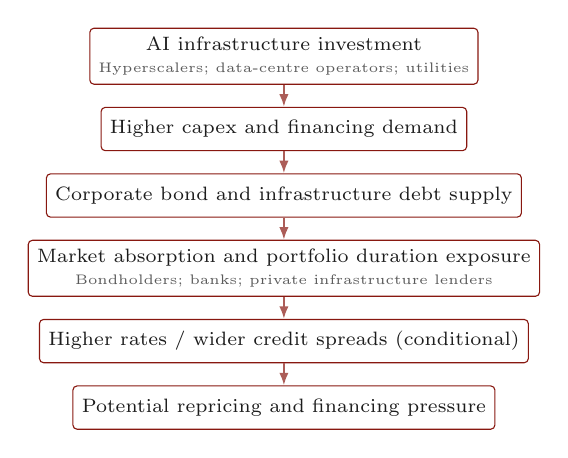
\begin{tikzpicture}[
  font=\scriptsize,
  box/.style={draw=navy, rounded corners=1.5pt, align=center, inner sep=3.2pt,
    text=ink, fill=white, minimum height=0.55cm},
  arr/.style={-{Latex[length=1.6mm]}, thick, color=navy!70},
  note/.style={font=\tiny\color{muted}, align=left}
]
\node[box] (a) {AI infrastructure investment\\{\tiny\color{muted}Hyperscalers; data-centre operators; utilities}};
\node[box, below=0.28cm of a] (b) {Higher capex and financing demand};
\node[box, below=0.28cm of b] (c) {Corporate bond and infrastructure debt supply};
\node[box, below=0.28cm of c] (d) {Market absorption and portfolio duration exposure\\{\tiny\color{muted}Bondholders; banks; private infrastructure lenders}};
\node[box, below=0.28cm of d] (e) {Higher rates / wider credit spreads (conditional)};
\node[box, below=0.28cm of e] (f) {Potential repricing and financing pressure};
\draw[arr] (a) -- (b);
\draw[arr] (b) -- (c);
\draw[arr] (c) -- (d);
\draw[arr] (d) -- (e);
\draw[arr] (e) -- (f);
\end{tikzpicture}
\end{center}
\vspace{-0.15em}
{\scriptsize\color{muted}\textbf{Note:} Conceptual schematic only. Does not establish contagion, crowding out, or systemic crisis.\par}

\defsig{Figure~7 orders a possible sequence from AI infrastructure investment to higher capex, to corporate and infrastructure debt supply, to portfolio duration, and, only if financial conditions tighten, to wider spreads and financing pressure. The names in the boxes (hyperscalers, data-centre operators, utilities, bondholders, banks, private infrastructure lenders) identify where the exposure can sit. Arrows are organising devices, not estimated elasticities.}{The figure is a map for the channels below. It keeps transmission hypothetical. A tighter rates or spread environment can reprice long paper and raise the cost of the next dollar of capex. The figure does not say that outcome is underway, and it does not say that stress at one issuer becomes stress for the credit market as a whole.}

\vspace{0.2em}

\begin{enumerate}[leftmargin=1.2em,itemsep=0.22em]
  \item \textbf{Supply and absorption.} Rapid long-dated issuance requires duration-constrained buyers. Wider new-issue spreads relative to rating-bucket OAS (Exhibit~4) and AA-bucket widening (Appendix~A1) are contemporaneous pricing signals, not proof of causation.
  \item \textbf{Index and benchmark concentration.} Passive and benchmarked portfolios hold the names by construction. Duration-risk share already exceeds market-value weight (Exhibit~1).
  \item \textbf{Issuer funding requirements.} Capex near or above operating cash flow (Exhibit~3) links credit metrics to external funding during the build, with resilience most constrained at Oracle.
  \item \textbf{Rating migration.} Oracle's path from A3/A$+$ (2020 pricing) to Baa2/BBB$-$ (November~2026 pricing) shows how a single large weight can approach the IG floor. \src{2}
  \item \textbf{Duration repricing.} In the June--September~2026 episode of a $\ge$50\,bp rise in the 10-year, IG OAS widened slightly, unlike earlier episodes in the ICE window. \src{3}\src{4}
\end{enumerate}

Off-balance-sheet leases and project-finance structures sit outside the registered-bond sample. J.P.~Morgan AM estimates about \$1.1\,tn of uncommenced data-centre lease obligations across hyperscalers. \src{11} These channels identify potential transmission; they do not empirically prove contagion or an emerging systemic crisis.

\subsection{Lookthrough for portfolio construction}

AI-related credit does not sit in one sleeve. The same five issuers are large weights in equity indices, a rising share of investment-grade duration (Exhibit~1), and, through leases, utilities and project finance, a claim on banks and private infrastructure lenders (Figure~7). An allocation that is long US equities, long benchmark IG credit, and long digital-infrastructure private credit can hold the same cash-flow exposure more than once, with no single line item showing the overlap.

That is why channel lookthrough matters for portfolio construction and asset allocation. Benchmarked credit portfolios absorb the extra duration whether or not the manager has an active view on AI. Equity beta and IG duration can move together if the build slows, or if long rates and credit spreads reprice in the same window (Appendix Exhibit~A3 describes co-movement; it does not predict it). An issuer limit applied only inside the bond book misses equity and private-credit exposure to the same operating cash flows. Spread risk is also uneven inside the bond sleeve: Table~2 concentrates at-issue DTS in Meta and Oracle, while Table~1 shows that only Oracle combines negative free cash flow with elevated leverage.

A practical allocation question follows. How much of the risk budget is already used by hyperscaler duration? How much incremental spread risk sits in the weaker funding profiles? Would adding more AI-linked credit, in public bonds or in private infrastructure, stack exposure the portfolio already holds through the equity index? This note does not assign weights. It identifies the exposures an allocation process should see before treating hyperscaler bonds as a separate, diversifying credit.

% =============================================================================
\section{Limitations}
% =============================================================================

\paragraph{What this outlook measures}
This note is an exploratory research outlook. It uses an original dataset of SEC-registered issuance and validated pricing terms, point-in-time 10-K/10-Q fundamentals, and FRED market series through 13~November~2026. Index duration-risk shares are published estimates (Bloomberg via bfinance). \src{10} At-issue durations, DTS and DV01 describe verified new issues. \src{2} Bracketed numbers cite Sources and References.

\paragraph{What it does not}
Exact index-level DTS contributions require licensed constituent files. Private (144A) bonds, term loans and project finance are missing, so issuance is a lower bound. Fiscal year-ends differ across issuers; TTM is the preferred common window. New-issue Treasury spreads and index OAS are related measures with different constructions. Scenario results are first-order illustrations, not forecasts of realised losses.

\vspace{0.15em}
{\scriptsize\color{muted}\textbf{Next data steps.}
(1)~Index constituent files for exact market-value, duration and DTS shares.
(2)~TRACE secondary spreads around deal days.
(3)~144A and private-placement coverage.
(4)~A rating-action event study.
(5)~Note-level maturity tables for the non-Oracle issuers.}

% =============================================================================
\section{Research summary}
% =============================================================================

This outlook asked whether hyperscaler debt contributes disproportionately to interest-rate sensitivity in U.S.\ investment-grade portfolios relative to its index market-value weight, and what explains that exposure.

On published Bloomberg-based estimates, the answer is yes for interest-rate duration, with a precise meaning of ``disproportionate.'' As of about September~2026, Amazon, Alphabet, Microsoft, Meta and Oracle were 4.85\% of Bloomberg US Corporate Index market value and 6.3\% of its duration risk, versus 2.67\% and 3.6\% at end-2024. \src{10} Both the weight and the duration share increased. The relative multiple did not. It remained about 1.3$\times$. The exposure is larger in dollars of rate risk. It is not a widening of sensitivity per dollar of market value.

Three facts explain the level of that exposure. Registered issuance scaled from \$14\,bn in 2023 to \$284\,bn in 2026, and duration supply grew through volume rather than longer average tenors (Exhibit~2). The new USD paper is long: 8.9~years at pricing, against 6.4~years for the index (Exhibit~1, Table~2). Capex now absorbs nearly all operating cash flow, so the supply is tied to an investment cycle rather than to a one-off refinancing (Exhibit~3). Resilience is not uniform. Oracle combines higher leverage, thinner coverage and negative free cash flow. Amazon is free-cash-flow negative with low leverage. Alphabet, Meta and Microsoft still self-fund, with less spare cash than earlier in the cycle (Table~1).

What the research does not establish matters as much as what it does. Spread gaps versus rating-bucket OAS have widened, especially for Oracle and Meta, but they are indicative comparisons, not measured concessions or an AI-specific premium (Exhibit~4). Near-term maturities remain modest beside the long paper issued (Exhibit~5). Hypothetical shocks show larger mark-to-market sensitivity on the 2025--26 book than on the index (Exhibit~6, Table~3); they are not forecasts. Leases and project finance sit outside the registered sample, so bond totals are a lower bound on financing.

For portfolio construction, the implication is lookthrough: benchmark credit already carries more duration from these five names than their weight implies, and the same cash flows can sit in equities, banks, utilities and private infrastructure. The evidence shows growing long-duration supply and uneven funding needs, not a refinancing crisis or contagion. The open question is whether demand and issuer flexibility can keep absorbing this cycle if conditions tighten. This outlook documents that question and does not recommend a position.
% =============================================================================
\appendix
\clearpage
\section*{Appendix}
\addcontentsline{toc}{section}{Appendix}

\noindent{\footnotesize\color{muted}Appendix exhibits provide supporting market context for the main findings. Each figure is defined below with panel descriptions, sources and interpretive limits.}

\vspace{0.35em}
\paragraph{Exhibit A1 definition}
Panel~(a) shows 10-year and 30-year Treasury constant-maturity yields. Panel~(b) shows ICE BofA AA, A and BBB option-adjusted spreads. Panel~(c) shows the A minus AA OAS differential, with a 21-day moving average. The shaded window (October~2025 onward) marks a descriptive period of heavy hyperscaler registered issuance and is not a causal identification window.

\exhibitblock{0.96}{appendixA1_rating_spreads.pdf}{%
  Exhibit A1: AA spreads widened relative to A and BBB through the supply wave}{%
  \textbf{Source:} FRED DGS10, DGS30 \src{3}; BAMLC0A2CAA, BAMLC0A3CA, BAMLC0A4CBBB (ICE via FRED) \src{4}. Daily, 13-Nov-2023 to 11-Nov-2026.\\
  \textbf{Note:} Supports the market-pricing discussion in Exhibit~4. Compression of A$-$AA OAS is an observed pricing fact, not proof of an AI-specific risk premium.}

\defsig{Panel~(a) is the 10-year and 30-year Treasury constant-maturity yield. Panel~(b) is ICE BofA AA, A and BBB option-adjusted spreads. Panel~(c) is the A OAS minus the AA OAS, with a 21-day moving average. The shaded window from October~2025 is a descriptive marker for heavy hyperscaler registered issuance. It is not a treatment window in a causal design. The ICE series on FRED begin 13~November~2023.}{The exhibit matters for Exhibit~4 because four of the five issuers price in or near the AA complex. AA OAS rose relative to A and BBB over the supply wave, and the A$-$AA gap compressed from about 21\,bp in 3Q25 to about 9\,bp in 3Q26. That is consistent with more AA-rated supply being absorbed. It does not prove that hyperscaler issuance caused the move. Treasury yields in panel~(a) are the rate backdrop against which those spread changes should be read.}

\clearpage
\paragraph{Exhibit A2 definition}
Panel~(a) places the hyperscaler supply wave in a longer Treasury-yield history. Panel~(b) compares Moody's seasoned Baa$-$10Y (long history) with ICE IG, BBB and AA OAS (available on FRED from 13~November~2023). Panel~(c) shows the Chicago Fed NFCI; positive readings indicate tighter-than-average financial conditions.

\nopagebreak
\exhibitblock{0.96}{appendixA2_rates_spreads_conditions.pdf}{%
  Exhibit A2: Treasury yields, IG spreads and financial conditions, Jan-2018 to Nov-2026}{%
  \textbf{Source:} FRED DGS2, DGS10, DGS30 \src{3}; BAA10Y \src{5}; BAMLC0A0CM, BAMLC0A4CBBB, BAMLC0A2CAA \src{4}; NFCI \src{6}.\\
  \textbf{Note:} ICE OAS series on FRED begin 13-Nov-2023. Moody's Baa$-$10Y is a long-history yield-spread proxy, not an OAS.}

\defsig{Panel~(a) is the 2-year, 10-year and 30-year Treasury constant-maturity yield from 2018. Panel~(b) places Moody's seasoned Baa corporate yield minus the 10-year Treasury, which has a long history, next to ICE IG, BBB and AA OAS, which FRED carries only from 13~November~2023. Panel~(c) is the Chicago Fed National Financial Conditions Index. Positive NFCI readings mean tighter-than-average financial conditions. The vertical marker in panel~(b) is the start of the ICE sample, not an economic event.}{The exhibit puts the 2025--26 supply wave in a longer rates and conditions history. Treasury yields are well above the 2020--21 lows, which is the backdrop for long-duration price sensitivity in Exhibit~6. ICE spreads, over the short window available, are tight relative to the 2020 spike in the Moody's series. NFCI has been easier than average for most of the recent window. The significance is context: the build-out has been financed in conditions that are not historically tight. A shift toward tighter NFCI, higher long yields, or wider OAS would change the absorption question in Section~8. The chart does not forecast that shift.}

\clearpage
\paragraph{Exhibit A3 definition}
The chart shows a 126-business-day rolling correlation of daily first differences between the 10-year Treasury yield and (i)~Moody's Baa$-$10Y and (ii)~ICE IG OAS. Correlation describes co-movement of changes; it does not identify causation or predict future episodes.

\exhibitblock{0.94}{appendixA3_rolling_correlation.pdf}{%
  Exhibit A3: Rolling six-month correlation of 10Y yield changes and credit-spread changes}{%
  \textbf{Source:} Author calculations based on FRED DGS10, BAA10Y and ICE IG OAS \src{3}\src{4}\src{5}.\\
  \textbf{Note:} 126-business-day window of daily first differences. Supports the rates-and-duration discussion in Credit-market considerations.}

\defsig{The chart is a 126-business-day rolling correlation of daily changes in the 10-year Treasury yield with daily changes in two spread measures: Moody's Baa$-$10Y, and, once the series exists, ICE IG OAS. Correlation here is co-movement of changes. A positive reading means yields and spreads tended to rise together over that window. A negative reading means they tended to move in opposite directions.}{The exhibit matters for the portfolio point in Section~8. If rates and spreads rise together, long hyperscaler bonds are hit on both the rate leg and the spread leg of Exhibit~6 at the same time, and an equity sleeve tied to the same issuers may not diversify that shock. If they move in opposite directions, the two legs can offset. The sample is short, especially for ICE, and the correlation changes sign across windows. It describes history. It does not identify a stable regime and it does not predict the next one.}

% =============================================================================
\clearpage
\section*{Sources and References}
\addcontentsline{toc}{section}{Sources and References}

\noindent{\scriptsize\color{muted}Numbered citations in the text and exhibit notes refer to the entries below. Exhibit source lines identify the specific series or filings used in each chart.}

\vspace{0.4em}
\noindent{\headingfont\footnotesize\bfseries\color{navy}A.\ Primary Financial Disclosures}\\[0.3em]
\begin{enumerate}[leftmargin=1.25em,itemsep=0.38em,parsep=0.05em,topsep=0em,label={\scriptsize\bfseries\color{navy}[\arabic*]}]
  \item {\scriptsize\textbf{U.S.\ Securities and Exchange Commission (SEC).} EDGAR Company Facts API; Forms 10-K and 10-Q for Amazon, Alphabet, Microsoft, Meta Platforms and Oracle. Retrieved 13~November~2026.
  \sourcelink{https://www.sec.gov/search-filings/edgar-application-programming-interfaces}{https://www.sec.gov/search-filings/edgar-application-programming-interfaces}}
  \item {\scriptsize\textbf{U.S.\ Securities and Exchange Commission (SEC).} EDGAR final prospectus supplements (424B2/424B5), free writing prospectuses (FWP), and debt offering term sheets. Retrieved 13~November~2026.
  \sourcelink{https://www.sec.gov/edgar/search/}{https://www.sec.gov/edgar/search/}}
\end{enumerate}

\vspace{0.35em}
\noindent{\headingfont\footnotesize\bfseries\color{navy}B.\ Market and Macroeconomic Data}\\[0.3em]
\begin{enumerate}[leftmargin=1.25em,itemsep=0.38em,parsep=0.05em,topsep=0em,resume,label={\scriptsize\bfseries\color{navy}[\arabic*]}]
  \item {\scriptsize\textbf{Federal Reserve Bank of St.\ Louis (FRED).} U.S.\ Treasury Constant Maturity Rates (DGS2, DGS5, DGS10, DGS30).
  \sourcelink{https://fred.stlouisfed.org/series/DGS10}{https://fred.stlouisfed.org/series/DGS10}}
  \item {\scriptsize\textbf{ICE Data Indices, LLC, via FRED.} ICE BofA U.S.\ Corporate OAS: BAMLC0A0CM (IG), BAMLC0A2CAA (AA), BAMLC0A3CA (A), BAMLC0A4CBBB (BBB), BAMLH0A0HYM2 (HY). Subject to vendor distribution window.
  \sourcelink{https://fred.stlouisfed.org/series/BAMLC0A0CM}{https://fred.stlouisfed.org/series/BAMLC0A0CM}}
  \item {\scriptsize\textbf{Moody's, via FRED.} Seasoned Corporate Bond Yield Spreads (BAA10Y, AAA10Y).
  \sourcelink{https://fred.stlouisfed.org/series/BAA10Y}{https://fred.stlouisfed.org/series/BAA10Y}}
  \item {\scriptsize\textbf{Federal Reserve Bank of Chicago, via FRED.} National Financial Conditions Index (NFCI).
  \sourcelink{https://fred.stlouisfed.org/series/NFCI}{https://fred.stlouisfed.org/series/NFCI}}
  \item {\scriptsize\textbf{Federal Reserve Board, via FRED.} H.10 FX and Effective Federal Funds Rate (DEXUSEU, DEXUSUK, DEXCAUS, DEXJPUS, DFF).
  \sourcelink{https://fred.stlouisfed.org/series/DEXUSEU}{https://fred.stlouisfed.org/series/DEXUSEU}}
  \item {\scriptsize\textbf{SIFMA.} Research Quarterly: Fixed Income Issuance and Trading (4Q2024, 4Q2025, 3Q2026).\\[0.1em]
  {\footnotesize\color{ink}\href{https://www.sifma.org/resources/research/research-quarterly-fixed-income-issuance-and-trading/}{\texttt{https://www.sifma.org/resources/research/}}\newline
  \href{https://www.sifma.org/resources/research/research-quarterly-fixed-income-issuance-and-trading/}{\texttt{research-quarterly-fixed-income-issuance-and-trading/}}}}
  \item {\scriptsize\textbf{SIFMA.} U.S.\ Corporate Bonds Statistics.\\[0.1em]
  {\footnotesize\color{ink}\href{https://www.sifma.org/resources/research/statistics/us-corporate-bonds-statistics/}{\texttt{https://www.sifma.org/resources/research/statistics/}}\newline
  \href{https://www.sifma.org/resources/research/statistics/us-corporate-bonds-statistics/}{\texttt{us-corporate-bonds-statistics/}}}}
\end{enumerate}

\vspace{0.35em}
\noindent{\headingfont\footnotesize\bfseries\color{navy}C.\ Institutional Research and Market Publications}\\[0.3em]
\begin{enumerate}[leftmargin=1.25em,itemsep=0.38em,parsep=0.05em,topsep=0em,resume,label={\scriptsize\bfseries\color{navy}[\arabic*]}]
  \item {\scriptsize\textbf{bfinance (2026).} ``AI, hyperscalers and corporate bond indices: signal or narrative?'' Xavier Blaiteau, 28~October~2026. Bloomberg index weights and duration exposure (constituent files not accessed).\\[0.1em]
  {\footnotesize\color{ink}\href{https://www.bfinance.com/insights/ai-hyperscalers-and-corporate-bond-indices-signal-or-narrative}{\texttt{https://www.bfinance.com/insights/}}\newline
  \href{https://www.bfinance.com/insights/ai-hyperscalers-and-corporate-bond-indices-signal-or-narrative}{\texttt{ai-hyperscalers-and-corporate-bond-indices-signal-or-narrative}}}}
  \item {\scriptsize\textbf{J.P.\ Morgan Asset Management (2026).} ``Hyperscalers: Now also a credit story.'' Jorn Veeneman, 20~August~2026.\\[0.1em]
  {\footnotesize\color{ink}\href{https://am.jpmorgan.com/be/en/asset-management/institutional/insights/market-insights/market-updates/on-the-minds-of-investors/hyperscaler-debt-issuance-ai-buildout/}{\texttt{https://am.jpmorgan.com/be/en/asset-management/}}\newline
  \href{https://am.jpmorgan.com/be/en/asset-management/institutional/insights/market-insights/market-updates/on-the-minds-of-investors/hyperscaler-debt-issuance-ai-buildout/}{\texttt{institutional/insights/market-insights/market-updates/}}\newline
  \href{https://am.jpmorgan.com/be/en/asset-management/institutional/insights/market-insights/market-updates/on-the-minds-of-investors/hyperscaler-debt-issuance-ai-buildout/}{\texttt{on-the-minds-of-investors/hyperscaler-debt-issuance-ai-buildout/}}}}
\end{enumerate}

\vspace{0.4em}
\noindent{\scriptsize\color{muted}Author calculations are based on the primary sources above, principally SEC EDGAR \src{1}\src{2} and FRED series \src{3}--\src{7}. Full source registry and validation diagnostics: \texttt{research/}, \texttt{outputs/diagnostics/}.}

\end{document}
